\documentclass{article}

\usepackage{tikz}

\newcommand{\Rubik}{
    \draw[black, thick] (0,0) -- (2.598,1.5);
    \draw[black, thick] (0,0) -- (-2.598,1.5);
    \draw[black, thick] (0,0) -- (0,-3);
    \draw[black, thick] (0,-3) -- (2.598,-1.5);
    \draw[black, thick] (0,-3) -- (-2.598,-1.5);
    \draw[black, thick] (0,-2) -- (2.598,-0.5);
    \draw[black, thick] (0,-2) -- (-2.598,-0.5);
    \draw[black, thick] (0,-1) -- (2.598,0.5);
    \draw[black, thick] (0,-1) -- (-2.598,0.5);
    \draw[black, thick] (2.598,-1.5) -- (2.598,1.5);
    \draw[black, thick] (-2.598,-1.5) -- (-2.598,1.5);
    \draw[black, thick] (0,3) -- (2.598,1.5);
    \draw[black, thick] (0,3) -- (-2.598,1.5);
    \draw[black, thick] (0.867,0.5) -- (0.867,-2.5);
    \draw[black, thick] (1.732,1) -- (1.732,-2);
    \draw[black, thick] (-0.867,0.5) -- (-0.867,-2.5);
    \draw[black, thick] (-1.732,1) -- (-1.732,-2);
    \draw[black, thick] (-0.867,0.5) -- (1.732,2);
    \draw[black, thick] (-1.732,1) -- (0.867,2.5);
    \draw[black, thick] (0.867,0.5) -- (-1.732,2);
    \draw[black, thick] (1.732,1) -- (-0.867,2.5);
}

\begin{document}

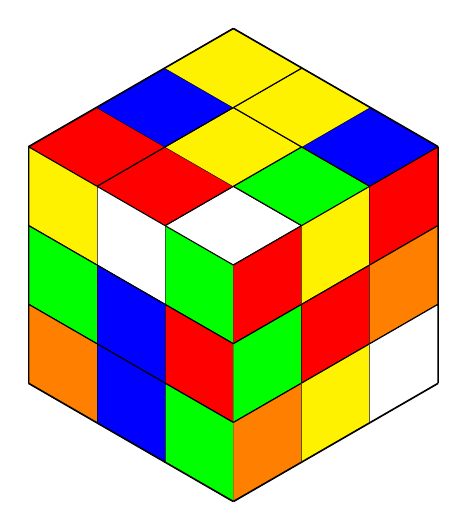
\begin{tikzpicture}
    \Rubik
    \draw [fill=white, draw=black] (0,0) -- (0.867,0.5) -- (0,1) -- (-0.867,0.5); 
    \draw [fill=red, draw=black] (-0.867,0.5) -- (0,1) -- (-0.867,1.5) -- (-1.732,1); 
    \draw [fill=red, draw=black] (-1.732,1) -- (-0.867,1.5) -- (-1.732,2) -- (-2.598,1.5);
    \draw [fill=green, draw=black] (0.867,0.5) -- (0,1) -- (0.867,1.5) -- (1.732,1);  
    \draw [fill=yellow, draw=black] (0,1) -- (0.867,1.5) -- (0,2) -- (-0.867,1.5); 
    \draw [fill=blue, draw=black] (-0.867,1.5) -- (0,2) -- (-0.867,2.5) -- (-1.732,2); 
    \draw [fill=blue, draw=black] (1.732,1) -- (0.867,1.5) -- (1.732,2) -- (2.598,1.5);
    \draw [fill=yellow, draw=black] (0.867,1.5) -- (0,2) -- (0.867,2.5) -- (1.732,2);
    \draw [fill=yellow, draw=black] (0,2) -- (0.867,2.5) -- (0,3) -- (-0.867,2.5);
    
    \draw [fill=green, draw=black] (0,0) -- (-0.867,0.5) -- (-0.867,-0.5) -- (0,-1); 
    \draw [fill=red, draw=black] (0,-1) -- (-0.867,-0.5) -- (-0.867,-1.5) -- (0,-2); 
    \draw [fill=green, draw=black] (0,-2) -- (-0.867,-1.5) -- (-0.867,-2.5) -- (0,-3); 
    \draw [fill=white, draw=black] (-0.867,0.5) -- (-1.732,1) -- (-1.732,0) -- (-0.867,-0.5); 
    \draw [fill=blue, draw=black] (-0.867,-0.5) -- (-1.732,0) -- (-1.732,-1) -- (-0.867,-1.5); 
    \draw [fill=blue, draw=black] (-0.867,-1.5) -- (-1.732,-1) -- (-1.732,-2) -- (-0.867,-2.5);
    \draw [fill=yellow, draw=black] (-1.732,1) -- (-2.598,1.5) -- (-2.598,0.5) -- (-1.732,0);
    \draw [fill=green, draw=black] (-1.732,0) -- (-2.598,0.5) -- (-2.598,-0.5) -- (-1.732,-1);
    \draw [fill=orange, draw=black] (-1.732,-1) -- (-2.598,-0.5) -- (-2.598,-1.5) -- (-1.732,-2);

    \draw [fill=red, draw=black] (0,0) -- (0.867,0.5) -- (0.867,-0.5) -- (0,-1); 
    \draw [fill=green, draw=black] (0,-1) -- (0.867,-0.5) -- (0.867,-1.5) -- (0,-2); 
    \draw [fill=orange, draw=black] (0,-2) -- (0.867,-1.5) -- (0.867,-2.5) -- (0,-3); 
    \draw [fill=yellow, draw=black] (0.867,0.5) -- (1.732,1) -- (1.732,0) -- (0.867,-0.5); 
    \draw [fill=red, draw=black] (0.867,-0.5) -- (1.732,0) -- (1.732,-1) -- (0.867,-1.5); 
    \draw [fill=yellow, draw=black] (0.867,-1.5) -- (1.732,-1) -- (1.732,-2) -- (0.867,-2.5);
    \draw [fill=red, draw=black] (1.732,1) -- (2.598,1.5) -- (2.598,0.5) -- (1.732,0);
    \draw [fill=orange, draw=black] (1.732,0) -- (2.598,0.5) -- (2.598,-0.5) -- (1.732,-1);
    \draw [fill=white, draw=black] (1.732,-1) -- (2.598,-0.5) -- (2.598,-1.5) -- (1.732,-2);
\end{tikzpicture}

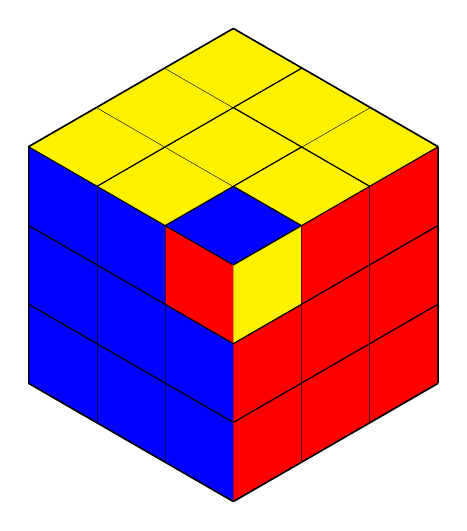
\begin{tikzpicture}
    \Rubik
    \draw [fill=blue, draw=black] (0,0) -- (0.867,0.5) -- (0,1) -- (-0.867,0.5); 
    \draw [fill=yellow, draw=black] (-0.867,0.5) -- (0,1) -- (-0.867,1.5) -- (-1.732,1); 
    \draw [fill=yellow, draw=black] (-1.732,1) -- (-0.867,1.5) -- (-1.732,2) -- (-2.598,1.5);
    \draw [fill=yellow, draw=black] (0.867,0.5) -- (0,1) -- (0.867,1.5) -- (1.732,1);  
    \draw [fill=yellow, draw=black] (0,1) -- (0.867,1.5) -- (0,2) -- (-0.867,1.5); 
    \draw [fill=yellow, draw=black] (-0.867,1.5) -- (0,2) -- (-0.867,2.5) -- (-1.732,2); 
    \draw [fill=yellow, draw=black] (1.732,1) -- (0.867,1.5) -- (1.732,2) -- (2.598,1.5);
    \draw [fill=yellow, draw=black] (0.867,1.5) -- (0,2) -- (0.867,2.5) -- (1.732,2);
    \draw [fill=yellow, draw=black] (0,2) -- (0.867,2.5) -- (0,3) -- (-0.867,2.5); 

    
    \draw [fill=red, draw=black] (0,0) -- (-0.867,0.5) -- (-0.867,-0.5) -- (0,-1); 
    \draw [fill=blue, draw=black] (0,-1) -- (-0.867,-0.5) -- (-0.867,-1.5) -- (0,-2); 
    \draw [fill=blue, draw=black] (0,-2) -- (-0.867,-1.5) -- (-0.867,-2.5) -- (0,-3); 
    \draw [fill=blue, draw=black] (-0.867,0.5) -- (-1.732,1) -- (-1.732,0) -- (-0.867,-0.5); 
    \draw [fill=blue, draw=black] (-0.867,-0.5) -- (-1.732,0) -- (-1.732,-1) -- (-0.867,-1.5); 
    \draw [fill=blue, draw=black] (-0.867,-1.5) -- (-1.732,-1) -- (-1.732,-2) -- (-0.867,-2.5);
    \draw [fill=blue, draw=black] (-1.732,1) -- (-2.598,1.5) -- (-2.598,0.5) -- (-1.732,0);
    \draw [fill=blue, draw=black] (-1.732,0) -- (-2.598,0.5) -- (-2.598,-0.5) -- (-1.732,-1);
    \draw [fill=blue, draw=black] (-1.732,-1) -- (-2.598,-0.5) -- (-2.598,-1.5) -- (-1.732,-2);

    \draw [fill=yellow, draw=black] (0,0) -- (0.867,0.5) -- (0.867,-0.5) -- (0,-1); 
    \draw [fill=red, draw=black] (0,-1) -- (0.867,-0.5) -- (0.867,-1.5) -- (0,-2); 
    \draw [fill=red, draw=black] (0,-2) -- (0.867,-1.5) -- (0.867,-2.5) -- (0,-3); 
    \draw [fill=red, draw=black] (0.867,0.5) -- (1.732,1) -- (1.732,0) -- (0.867,-0.5); 
    \draw [fill=red, draw=black] (0.867,-0.5) -- (1.732,0) -- (1.732,-1) -- (0.867,-1.5); 
    \draw [fill=red, draw=black] (0.867,-1.5) -- (1.732,-1) -- (1.732,-2) -- (0.867,-2.5);
    \draw [fill=red, draw=black] (1.732,1) -- (2.598,1.5) -- (2.598,0.5) -- (1.732,0);
    \draw [fill=red, draw=black] (1.732,0) -- (2.598,0.5) -- (2.598,-0.5) -- (1.732,-1);
    \draw [fill=red, draw=black] (1.732,-1) -- (2.598,-0.5) -- (2.598,-1.5) -- (1.732,-2);
\end{tikzpicture}

\newpage
\section{Appendix}

\begin{center}
    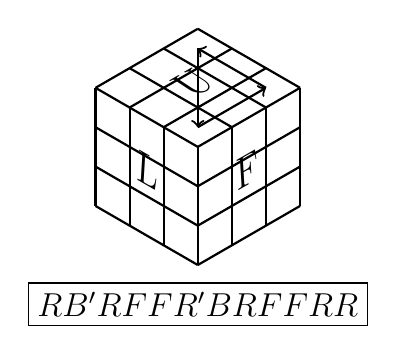
\begin{tikzpicture}[scale=0.5]
        \Rubik
        \draw[->, thick, black] (0,0.5) -- (1.732,1.5);
        \draw[->, thick, black] (1.732,1.5) -- (0,2.5);
        \draw[->, thick, black] (0,2.5) -- (0,0.5);
        \draw (0,-2) -- (2.598,-0.5) node[midway,sloped,above,xslant=0.5,] {\Large{F}};
        \draw (0,-2) -- (-2.598,-0.5) node[midway,sloped,above,xslant=-0.5,] {\Large{L}};
        \draw (-0.867,0.5) -- (1.732,2) node[midway,sloped,above,xslant=-0.5,] {\Large{U}};
        \node at (0,-4) [rectangle, draw] {\large$RB'RFFR'BRFFRR$};
    \end{tikzpicture}
    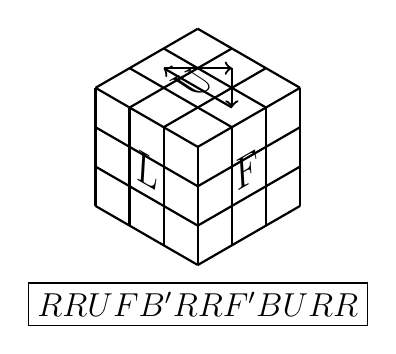
\begin{tikzpicture}[scale=0.5]
        \Rubik
        \draw[->, thick, black] (0.867,1) -- (-0.867,2);
        \draw[->, thick, black] (-0.867,2) -- (0.867,2);
        \draw[->, thick, black] (0.867,2) -- (0.867,1);
        \draw (0,-2) -- (2.598,-0.5) node[midway,sloped,above,xslant=0.5,] {\Large{F}};
        \draw (0,-2) -- (-2.598,-0.5) node[midway,sloped,above,xslant=-0.5,] {\Large{L}};
        \draw (-0.867,0.5) -- (1.732,2) node[midway,sloped,above,xslant=-0.5,] {\Large{U}};
        \node at (0,-4) [rectangle, draw] {\large$RRUFB'RRF'BURR$};
    \end{tikzpicture}
\end{center}

\begin{center}
    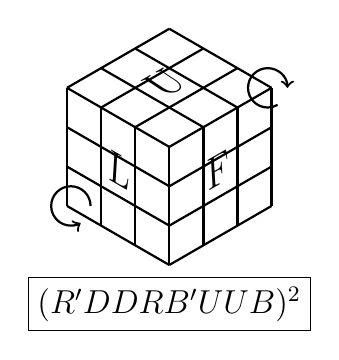
\begin{tikzpicture}[scale=0.5]
        \Rubik
        \draw[<-, thick, black] (3,1.5) arc(0:300:0.5);
        \draw[->, thick, black] (-2,-1.5) arc(0:300:0.5);
        \draw (0,-2) -- (2.598,-0.5) node[midway,sloped,above,xslant=0.5,] {\Large{F}};
        \draw (0,-2) -- (-2.598,-0.5) node[midway,sloped,above,xslant=-0.5,] {\Large{L}};
        \draw (-0.867,0.5) -- (1.732,2) node[midway,sloped,above,xslant=-0.5,] {\Large{U}};
        \node at (0,-4) [rectangle, draw] {\large$(R'DDRB'UUB)^2$};
    \end{tikzpicture}
    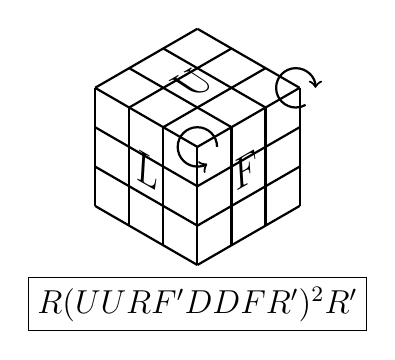
\begin{tikzpicture}[scale=0.5]
        \Rubik
        \draw[<-, thick, black] (3,1.5) arc(0:300:0.5);
        \draw[->, thick, black] (0.5,0) arc(0:300:0.5);
        \draw (0,-2) -- (2.598,-0.5) node[midway,sloped,above,xslant=0.5,] {\Large{F}};
        \draw (0,-2) -- (-2.598,-0.5) node[midway,sloped,above,xslant=-0.5,] {\Large{L}};
        \draw (-0.867,0.5) -- (1.732,2) node[midway,sloped,above,xslant=-0.5,] {\Large{U}};
        \node at (0,-4) [rectangle, draw] {\large$R(UURF'DDFR')^2R'$};
    \end{tikzpicture}
\end{center}

\begin{center}
    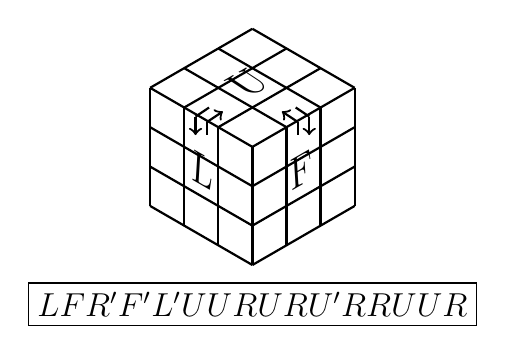
\begin{tikzpicture}[scale=0.5]
        \Rubik
        \draw[black, thick] (1.156,0.63) -- (1.156,0.3);
        \draw[->, black, thick] (1.156,0.63) -- (0.75,0.9);
        \draw[black, thick] (1.444,0.77) -- (1.1,1);
        \draw[->, black, thick] (1.444,0.77) -- (1.444,0.3);
        \draw[black, thick] (-1.156,0.63) -- (-1.156,0.3);
        \draw[->, black, thick] (-1.156,0.63) -- (-0.75,0.9);
        \draw[black, thick] (-1.444,0.77) -- (-1.1,1);
        \draw[->, black, thick] (-1.444,0.77) -- (-1.444,0.3);
        \draw (0,-2) -- (2.598,-0.5) node[midway,sloped,above,xslant=0.5,] {\Large{F}};
        \draw (0,-2) -- (-2.598,-0.5) node[midway,sloped,above,xslant=-0.5,] {\Large{L}};
        \draw (-0.867,0.5) -- (1.732,2) node[midway,sloped,above,xslant=-0.5,] {\Large{U}};
        \node at (0,-4) [rectangle, draw] {\large$LFR'F'L'UURURU'RRUUR$};
    \end{tikzpicture}
\end{center}



\begin{center}
    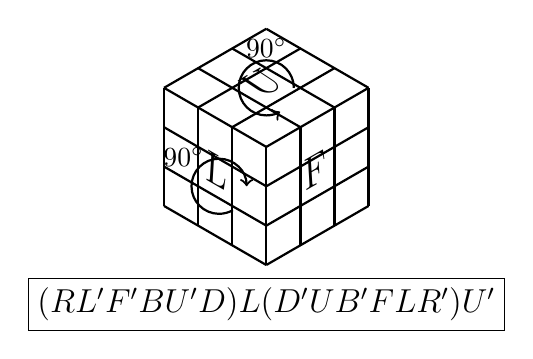
\begin{tikzpicture}[scale=0.5]
        \Rubik
        \draw[<-, thick, black] (-0.5,-1) arc(0:300:0.7);
        \draw[->, thick, black] (0.7,1.5) arc(0:300:0.7);
        \node at (-2.1,-0.25) {$90^\circ$};
        \node at (0,2.5) {$90^\circ$};
        \draw (0,-2) -- (2.598,-0.5) node[midway,sloped,above,xslant=0.5,] {\Large{F}};
        \draw (0,-2) -- (-2.598,-0.5) node[midway,sloped,above,xslant=-0.5,] {\Large{L}};
        \draw (-0.867,0.5) -- (1.732,2) node[midway,sloped,above,xslant=-0.5,] {\Large{U}};
        \node at (0,-4) [rectangle, draw] {\large$(RL'F'BU'D)L(D'UB'FLR')U'$};
    \end{tikzpicture}
    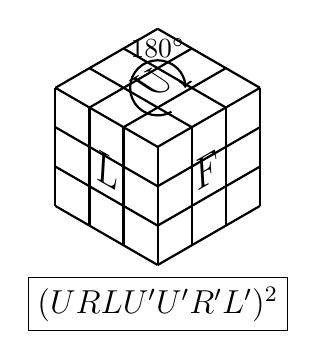
\begin{tikzpicture}[scale=0.5]
        \Rubik
        \draw[<-, thick, black] (0.7,1.5) arc(0:300:0.7);
        \node at (0,2.5) {$180^\circ$};
        \draw (0,-2) -- (2.598,-0.5) node[midway,sloped,above,xslant=0.5,] {\Large{F}};
        \draw (0,-2) -- (-2.598,-0.5) node[midway,sloped,above,xslant=-0.5,] {\Large{L}};
        \draw (-0.867,0.5) -- (1.732,2) node[midway,sloped,above,xslant=-0.5,] {\Large{U}};
        \node at (0,-4) [rectangle, draw] {\large$(URLU'U'R'L')^2$};
    \end{tikzpicture}
\end{center}



\end{document}
